\documentclass[11pt,letterpaper]{article}
\usepackage[lmargin=1in,rmargin=1in,tmargin=1in,bmargin=1in]{geometry}
\usepackage{../style/homework}
\usepackage{../style/commands}
\setbool{quotetype}{true} % True: Side; False: Under
\setbool{hideans}{true} % Student: True; Instructor: False

% -------------------
% Content
% -------------------
\begin{document}

\homework{1: Due 09/07}{I have no idea what I'm doing, but I know I'm doing it really, really well.}{Andy Dwyer, Parks and Recreation}

% Problem 1
\problem{10} A small tanker truck is depositing its gas at a storage facility. The tanker is carrying 11,600~gallons of gas and is emptying its tank at a rate of 528.3~gal/min. Let $G(t)$ denote the volume of gas, in thousands, left in the tanker $t$ minutes from now. 
	\begin{enumerate}[(a)]
	\item Explain why $G(t)$ is linear. 
	\item Find $G(t)$ and sketch it in the plot below. 
	\item Interpret the slope of $G(t)$.
	\item Interpret the $y$-intercept for $G(t)$.
	\item Find and interpret (if possible) the $x$-intercept for $G(t)$. 
	\end{enumerate}
	
	\vfill
	
	\[
	\fbox{
	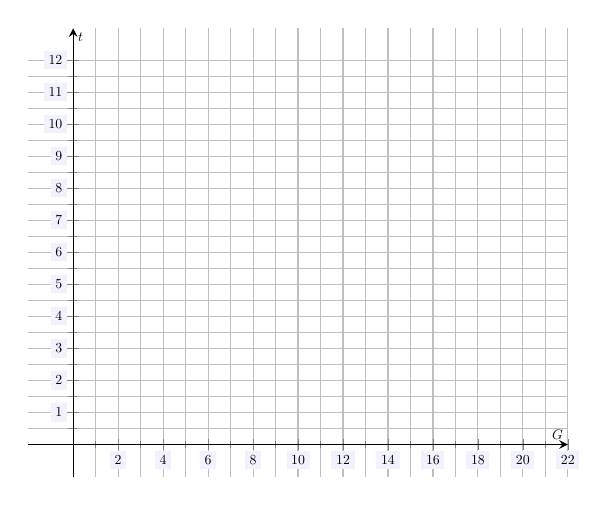
\begin{tikzpicture}[scale=1,every node/.style={scale=0.5}]
	\begin{axis}[
	grid=both,
	axis lines=middle,
	ticklabel style={fill=blue!5!white},
	xmin= -2, xmax=22,
	ymin= -1, ymax=13,
	xtick={0,2,...,22},
	ytick={0,1,2,...,12},
	minor x tick num = 1,
	minor y tick num = 1,
	xlabel=\(G\),ylabel=\(t\),
	]
	\end{axis}
	\end{tikzpicture}
	}
	\] 



\newpage



% Problem 2
\problem{10} Compute the following:
	\begin{enumerate}[(a)]
	\item 83\% of 2,429
	\item 17\% of 94.2
	\item 121\% of 16
	\item 55 decreased by 27\%
	\item 430 increased by 60\%
	\item 38 increased by 130\%
	\end{enumerate}
	
	

\newpage



% Problem 3
\problem{10} Monty offers wellness classes at his spa. A session typically costs \$65; however, due to popularity, Monty is raising his prices. Over the next three months, he will raise his prices by 5\% each month. 
	\begin{enumerate}[(a)]
	\item How much will a wellness session cost at the end of the three months? Be sure to justify your answer. 
	\item Is your answer in (a) the same as raising the original price by 15\%? Explain. 
	\item If he simply made the price \$80, by what percentage did he increase the price from the original price?
	\item By what percentage would Monty have to increase his prices over the next three months so that the final cost of a wellness session would be the same as a single price increase of 20\% from the original cost?
	\end{enumerate}


\end{document}